%%
%% ****** ljmsamp.tex 13.06.2018 ******
%%
\documentclass[
11pt,%
tightenlines,%
twoside,%
onecolumn,%
nofloats,%
nobibnotes,%
nofootinbib,%
superscriptaddress,%
noshowpacs,%
centertags]%
{revtex4}
\usepackage{ljm}
\begin{document}

\titlerunning{Short form of the title} % for running heads
\authorrunning{First-Author at al.} % for running heads
%\authorrunning{First-Author, Second-Author} % for running heads

\title{Investigation of the Predictive Properties \\
 of Solving the Inverse Problem\\ of Identifying the Aquifer Model for an Oil Reservoir}
% Splitting into lines is performed by the command \\
% The title is written in accordance with the rules of capitalization.

\author{\firstname{V.~P.}~\surname{Kosyakov}}
\email[E-mail: ]{lik.24@yandex.ru}
\affiliation{Tyumen Branch of Khristianovich Institute of Theoretical and Applied Mechanics SB RAS, Taymirskaya Str. 74, 625026, Tyumen, Russia}


\received{March 02, 2020} % The date of receipt to the editor, i.e. December 06, 2017


\begin{abstract} % You shouldn't use formulas and citations in the abstract.
When modeling the development of an oil field, one of the most important steps is to solve the inverse problem, the solution of which, as a rule, is to select the model parameters for the best tuning to the development history. However, the purpose of modeling is not only to repeat development indicators on the historical period, but also to obtain a reliable forecast of the behavior of the simulated object in the future. Therefore, from the point of view of the long-term forecast characteristics of the model, it is necessary to perform not only parametric, but also structural identification of the model.
In this paper, an example of solving the problem of structural and parametric identification of an aquifer circuit model (aquifer) for modeling the development of an oil field is a study of their predicted characteristics. It is shown that, as a result of structural and parametric identification of the model, its predictive properties can be significantly improved compared with the case of conventional parametric identification.
\end{abstract}

\subclass{12345, 54321} % Enter 2010 Mathematics Subject Classification.

\keywords{inverse problem, structural-parametric identification, numerical modeling, aquifer} % Include keywords separeted by comma.

\maketitle

% Text of article starts here.

\section{Introduction}

In the process of modeling the development of an oil field, one of the most important steps is to solve the inverse problem. The solution of which, as a rule, is to select the model parameters for the best tuning to the development history. In turn, the purpose of modeling is not only to repeat development indicators on the historical period, but also to obtain a reliable forecast of the behavior of the simulated object. The choice of a mathematical model is determined by the goals and objectives for the solution of which it will be used. In this case, the goal is to obtain a quality forecast. Based on the requirements of adaptation and forecasting problems, the identification problem consists in determining the structure and parameters of a mathematical model that provide a satisfactory description of historical data and have the best predictive characteristics.

To assess the predicted characteristics of the model, a breakdown of the historical period into 2 time intervals is often used: on the first, the model is adapted, and on the second, the forecast properties of the model are evaluated. It was shown in \cite{mus} that the best adaptation does not necessarily have the best predictive properties, which largely depend on the complexity of the chosen model. In addition, the predicted characteristics depend on the specific conditions (control parameters) of the model at the stages of adaptation and validation.

This paper presents a study of the dependence of the predicted characteristics of the model on the consistency of operating modes at the stages of adaptation and validation. Using the problem of identifying an aquifer model and adapting its parameters for an oil field as an example, the importance of structural identification from the point of view of the long-term forecast characteristics of the model is shown. The reservoir pressure, which characterizes the "energy" potential of the reservoir, acts as a predicted parameter. The aquifer model is important for the predictive characteristics of the model from the point of view of its energy state under conditions of intensive development of the \cite{kos} field, which includes depletion, drilling new wells, the formation of a reservoir pressure maintenance system, massive shutdown of wells, etc. d.

\section{MODEL}

To solve this problem, a two-dimensional mathematical model of single-phase filtration for a weakly compressible fluid \cite{bas} was used as a filtration model. To simulate the behavior of the aquifer, a set of 4 models of varying degrees of complexity \cite{dake}, \cite{fet} was used. The complexity of the model is determined by the number of adjustable parameters. We denote by $F(P_ {aq}, P, \nu) $ the function describing the flow of fluid, which generally depends on the mean pressure in the aquifer $P_{aq}$, pressure in the computational domain $P$ and on the parameter vector $\nu$. The study was conducted for four aquifer models:
\begin{enumerate}
	\item model allowing to describe the behavior of an isolated object, there are no adaptable parameters (M1);
	\item model of constant pressure on the supply circuit (aquifer of infinite volume), has one adjustable parameter (M2);
	\item finite volume aquifer model, has 2 adjustable parameters (M3);
	\item final volume aquifer model with a remote power supply circuit - 3 adjustable parameters (M4).
\end{enumerate}
Thus, the system of equations can be written in the following form:
\begin{equation} \label{fil}
\left\{\begin{array}{crl}
\triangledown\sigma\triangledown P = \beta^*h\frac{dP}{dt}+\delta(x,y)\\
q_{aq} = F(P,\nu)
\end{array}\right.
\end{equation}

\begin{equation} \label{bc}
\delta(x,y)  = \left\{\begin{array}{crl}
0\;???\;(x,y) \notin\ \Gamma_{in}\cup\Gamma_{out}\\
q_j\;???\;(x,y) \in \Gamma_{in}\\
q_{aq}\;???\;(x,y) \in \Gamma_{out}
\end{array}\right.
\end{equation}
\begin{equation*}
P(t=0) = P_{aq}(t=0) = P_0
\end{equation*}
where $\sigma$ is the hydraulic conductivity, $P$ is the reservoir pressure, $\beta^*$ is the effective compressibility, $h$ is the effective thickness, $q_j$ is the fluid flow in the $j$ well, $\Gamma_{in}$ is the set of coordinates of sources (wells), $\Gamma_{out}$ is the external boundary, $P_0$ is the reservoir pressure at the initial time $t=0$.

Aquifer models (M1-M4) can be described by the following equations:
\begin{equation}
q_{aq}=0
\end{equation}
\begin{equation}
q_{aq} = \lambda\sigma(P|_{\Gamma_{out}}-P_c)
\end{equation}
\begin{equation}
\beta^*V_{aq}\frac{dP_{aq}}{dt} = \lambda\oint_{\Gamma_{out}}\frac{\sigma}{h}(P-P_{aq})d\Gamma_{out}
\end{equation}
\begin{equation}
\beta^*V_{aq}\frac{dP_{aq}}{dt} =\lambda\oint_{\Gamma_{out}}\frac{\sigma}{h}(P-P_{aq})d\Gamma_{out} + \kappa(P_{aq}-P_c)
\end{equation}
where $V_{aq}$ is the volume of aquifer, $P_c$ is the pressure on the supply circuit ($P_c = P_0$), $P_{aq}$ is the pressure in the aquifer, $\lambda$ is the coefficient of productivity of the aquifer, $\kappa$ - remote zone productivity. Thus, the vector $\nu = [\lambda, V_{aq}, \kappa]$, for the aquifer model M4.

Using (\ref{fil} - \ref{bc}), the inverse problem is solved, which consists in minimizing the objective function $J$, which is MAPE (mean absolute percentage error). The arguments of the objective function are the actual and calculated values ??of the reservoir pressure at the points of location of the wells. The objective function is written as follows:
\begin{equation} \label{mape}
J=\frac{1}{N}\sum_{i=1}^N{\left\vert\frac{p_c^i-p_f^i}{p_f^i}\right\vert}\rightarrow min
\end{equation}
where $p_c$ is the calculated value of reservoir pressure, $p_f$ is the actual value, $N$ is the total number of measurements. The solution to the problem is found using the gradient optimization algorithm and consists in determining a set of model parameters corresponding to a minimum of $ J $ and satisfying the inequality constraints: $\nu_{min} \leq \nu \leq \nu_{max}$.

A custom parameter $a$ was introduced into the filtration model - a factor for hydraulic conductivity, thus in (\ref{fil}) $\sigma = a\cdot\sigma_0$, where $\sigma_0$ is the initial approximation for hydraulic conductivity, $a>0$. Therefore, to solve the adaptation problem, it will be necessary to determine the values of the parameter vector $u = [a, \nu]$ of length from 1 to 4. The value of the gradient of the objective function for the components can be written in the following form:
\begin{equation}
\frac{dJ}{du} = \frac{1}{N}\sum_{i=1}^N sgn\left(\frac{p_c^i-p_f^i}{p_f^i}\right)\frac{dp_c^i}{du}
\end{equation}
Thus, to solve the inverse problem, it is necessary that
\begin{equation} \label{rp}
	 \frac{dJ}{du} \rightarrow 0
\end{equation}
The solution to the direct (\ref{fil} - \ref{bc}) and inverse (\ref{rp}) problems was found numerically implicitly using a two-dimensional unstructured grid.


\section{Model}
As an example, the inverse problem of structural-parametric identification for an oil field was solved. To solve the problem, a data set is required (the size of the computational domain, the location of the wells and the development indicators for the wells: fluid flow and pressure), which was obtained using a synthetic hydrodynamic model. These data acted as "actual" values.

The layout of the wells and the legend are shown in the figure \ref{fig: map}.
% \ center {\ includegraphics [height = 6pc] {fig1.png}}
\begin{figure}
    \begin{minipage} [h] {0.69 \linewidth}
      \center{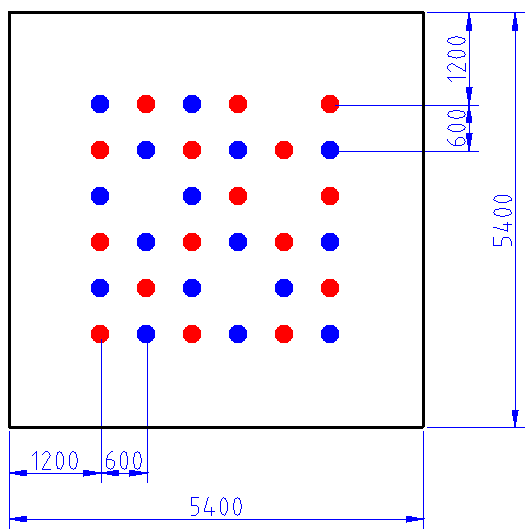
\includegraphics [width = 16pc]{fig1a.png} \\ (a)}
    \end{minipage} \hfill
    \begin{minipage} [h] {0.29 \linewidth}
      \center{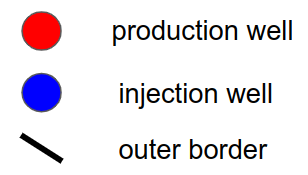
\includegraphics [width = 8pc]{fig1b.png} \\ (b)}
    \end{minipage}
    \caption{Schematic representation of the computational domain (a) and legend (b).}
    \label{fig: map}
\end{figure}
The field is developed using 16 producing and 16 injection wells. The development period is 10 years, the power circuit was "connected" along the perimeter of the computational domain. To solve the problem of structural-parametric identification, the time interval was divided into 3 parts of 72, 24, and 24 months, respectively:
\begin{enumerate}
	\item from 01-2000 to 12-2005 adaptation period;
	\item from 01-2006 to 12-2007 validation period;
	\item from 01-2008 to 12-2009 forecast period.
\end{enumerate}

At the adaptation time interval, the inverse problem is solved for all 4 models, with unknown parameters. On the validation interval, the predicted characteristics of the tuned model are evaluated, and a model with the best predictive characteristics is selected. In addition, the third interval was selected - the forecast interval, on which the behavior of the adapted model is evaluated with a significant change in the control parameters. The time interval for the adaptation phase was chosen in such a way that it included the phased commissioning of all wells and a stationary mode of operation was achieved. The validation phase also includes the stationary operation interval of the field.

For the forecasting phase, 3 operational scenarios were calculated for each model, and the behavior of the main development parameters was compared. The following scenarios were calculated: S0 - stationary operation mode, S1 - twofold decrease in the volume of the injected fluid, and S2 - twofold increase in the volume of the injected fluid compared to the scenario S0.

The figure \ref{fig:2din} shows the dynamics of the average reservoir pressure for the actual data (B is the base case) and all aquifer models (M1-M4 aquifer models). The \ref{fig: hist} histogram shows the value (\ref{mape}) for the adaptation (adp) and validation (val) intervals.
\begin{figure}
    \begin{minipage}[h]{0.48 \linewidth}
      \center{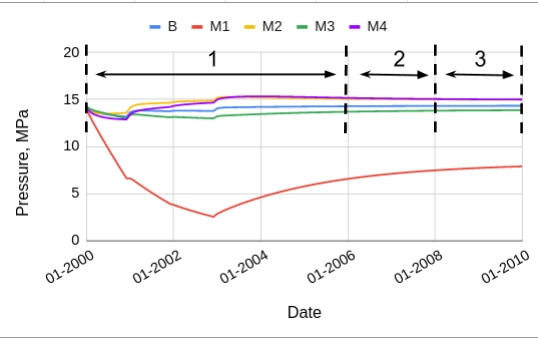
\includegraphics[height = 0.65 \linewidth] {fig2.png}}
      \caption{Dynamics of the average reservoir pressure for different models of the aquifer}
      \label{fig: din}
    \end{minipage} \hfill
    \begin{minipage}[h]{0.48 \linewidth}
      \center{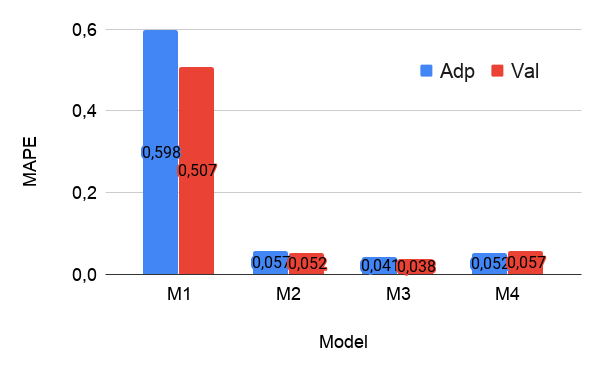
\includegraphics[height = 0.65 \linewidth] {fig3.png}}
      \caption{MAPE for the adaptation (adp) and validation (val) stages}
      \label{fig: hist}
    \end{minipage}
\end{figure}

It can be seen from the figures that the M1 model has the worst performance both at the adaptation stage and at the exam stage. The value of the objective function is approximately an order of magnitude greater than that of other models; therefore, the M1 model is the least suitable for describing the behavior of the modeled object and will not be used in further studies. The best characteristics for adaptation and validation are those of the M3 model. Models M2 and M4 have satisfactory values ??of the objective function. If we compare only these two models, then M4 describes the history better, and M2 has better predictive properties, so the choice of these two models must be carried out using some other criteria, such as BIC \cite{mus}.

In practice, as a rule, only the task of adaptation is solved and the choice of model is carried out expertly. Models are rejected mainly by the criterion of not exceeding the error inherent in various regulations (usually from 5 to 25\%). Correspondingly, the M2-M4 models, due to the relatively small difference in their indicators, can be equally likely selected as predictive models. Indeed, the most pronounced difference in pressure dynamics for different models is observed in the initial period ? when new wells are entered and stationary wells are operating. In stationary modes, the trends are generally similar, and models in stationary modes have similar predictive characteristics.

The behavior of the adapted model with a significant (extreme) change in the operating mode of wells implemented in scenarios S1 and S2 is interesting. Figure \ref{fig:2din} shows the dynamics of the average reservoir pressure for three models (M2-M4) under three development scenarios (S0-S2).
\begin{figure}
\center{ 
    \begin{minipage}[h]{0.32\linewidth}
      \center{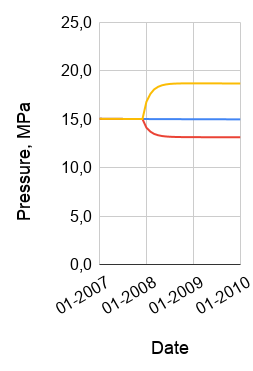
\includegraphics[height=1.5\linewidth]{fig4a.png} \\ (a)}
    \end{minipage} \hspace{0pt}
    \begin{minipage}[h]{0.32\linewidth}
      \center{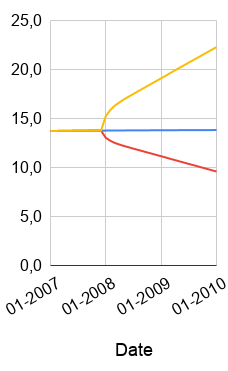
\includegraphics[height=1.5\linewidth]{fig4b.png} \\ (b)}
    \end{minipage} \hspace{0pt}
    \begin{minipage}[h]{0.32\linewidth}
      \center{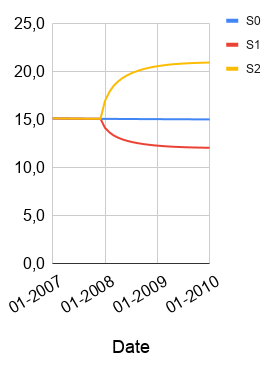
\includegraphics[height=1.5\linewidth]{fig4c.png} \\ (c)}
    \end{minipage} 
    \caption{Dynamics of average reservoir pressure for 3 aquifer models under 3 development scenarios, where a, b, and c correspond to M2, M3, and M4.}
    \label{fig:2din}
    }
\end{figure}
As can be seen from the graphs, the behavior of the models under the same scenarios is different (S1 and S2). The difference lies not only in the absolute values of the reservoir pressure, but also in the dynamics of its change. Accordingly, the forecast indicators of each model will differ significantly.

\section{CONCLUSIONS}

As a result of the study, it was shown that obtaining a satisfactory solution to the inverse problem can be achieved using models of varying degrees of complexity. In addition to the quality of tuning the model to the development history - the quality of adaptation, it is also necessary to evaluate its predictive properties. The validation procedure allows the selection of a model that has the best predictive characteristics. In addition, the work demonstrated that the quality of the forecast, in addition to the complexity of the model, depends on the similarity of development scenarios in which the model was adapted and validated. With a significant difference between the predicted modes and those on which the model was adjusted, the predicted properties of the model are sharply reduced. Upon receipt of the actual data, it is necessary to re-carry out the procedure of structurally parametric identification.

\section{FUNDING}
The study was performed by a grant from the Russian Foundation for Basic Research (project no. 18-29-10023).


%
\begin{thebibliography}{99}
\bibitem{mus} E. N. Musakaev, S. P. Rodionov, D. Y. Legostaev, V. P. Kosyakov,  �Parameter identification for sector filtration model of an oil reservoir with complex structure� // AIP Conference Proceedings 2125,030113 2009;

\bibitem{kos} V. P. Kosyakov, D. Y. Legostaev,  �Computational technology for solution of the reverse problem of filtration theory for oil fields with an aquifer� // AIP Conference Proceedings 2125,030112 2009;

\bibitem{bas} K. S. Basniev, N. M. Dmitriev, R. D. Kanevskaya, V. M. Maksimov. \textit{Underground hydromechanics}. M.-Izhevsk: Institute for Computer Research, 2006. [in Russian]

\bibitem{dake} L. P. Dake, \textit{Fundamentals of Reservoir Engineering} (Elsevier, Amsterdam, 1978).

\bibitem{fet} M. J. Fetkovich. A Simplifi ed approach to water infl ux calculations ? Finite aquifer systems. J. Pet. Tech. July 1971, vol. 23, is. 7, pp. 814-828.


\end{thebibliography}


\end{document}
